\chapter{Конструирование виртуальных мультиагентных подсетей}\label{ch:ch4}

\section{Конструирование Web-ресурсов}\label{sec:ch4/sect1}

\section{Типы виртуальных сетевых агентов}\label{sec:ch4/sect2}

\subsection{Index data structure, functionality and microservices in thematic virtual museums}\label{subsec:ch4/sec2/sub1}

\paragraph{1. Introduction.} Museum as nonprofit institution which responsible for preserving historical and cultural heritage, exhibit tangible and intangible to public is facing huge problem in digital era as mention in \cite{AnggaiBlekanovSergeev2014}. Museums institution are starting digitizing their collections and describe detail information in order to intensify their activities and present on the Internet as a part of public services. However, digital transformation is inevitable, museums institution must provide good impact, experiences and values to their visitors.

The thematic concept in virtual museum is one of the approaches we take in order to accelerate digital transformation of museums institution. We are combining virtual museum (VM) and information retrieval (IR) concepts in conducting information management, analytics, and focus on users-centric to enhance their experience by providing visitors’ information need within the virtual museums system.

In this research work we are preparing, investigating and conducting experiments on data access service, index construction, applying ranking algorithms and development of microservices in thematic virtual museums for speeding up disruptive innovation in museums institution.

\paragraph{2. Data crawling.}  In section 2 we will describe how this application data access crawling service get the content of web pages. This crawler service can take data from museums institution in text, Hypertext Markup Language (HTML), JavaScript Object Notation (JSON), or Extensible Markup Language (XML) form. We define specific web Uniform Resource Locator (URL) to crawl and run the service to obtain content pages. The crawler service maintains and run a job for specific website and not for general uses, because it ought to crawl based on characteristics of each page in those websites. As in our case we are getting the data from Registration Museum under Ministry of Education and Culture, Republic of Indonesia. There are two models web pages structure in order to get full museum collection pages as the following.

\begin{enumerate}
	\item List of collections. The crawler service directly accesses to the URL which contains list of museum collections. This URL address show 20 items per page and navigation page to identify how many pages still remain as previous or next page from the first to the end page. All URL retrieved from this page which identified as detail collection URL will be adding to download-queue.
	\item Detail of collection. This page contains detail collection information and it can be marked as end of page to be crawled. The information which contain on this page is name of museum institution, collection type, function, age, description and picture with a title.
\end{enumerate}

The crawler services automatically download the content page until all pages have been crawled. In order to prevent Internet network traffic, we are providing delay-time parameter to the crawler services, therefore this engine can be customizing to aggressive or polite crawler modes. The algorithm we are using on this task is Breadth First Search \cite{HassaanBurtscherPingali}, however the page of collection is not deep, therefore to download those pages the formula can be written as shown below:
\[
f(p) = \sum_{i = 1}^{n} \sum_{j = 1}^{m} \textit{dl }(\textit{page})
\]

\paragraph{3. Parsing data.} In this stage the service will parse data which has been obtained. There are two models we have been using in order to parsing data from crawler service, first we are directly parsing HTML format into Thermal VM (TVM) data schema, and second the parser service follow standard rule for data exchange. Parser service has developed for performing tasks in general, therefore data collections which obtained by crawler can be fully implemented on this service. We are using method as shown in Figure~\cref{fig:tvmMapping}.

\begin{figure}[ht]
	\centerfloat{
		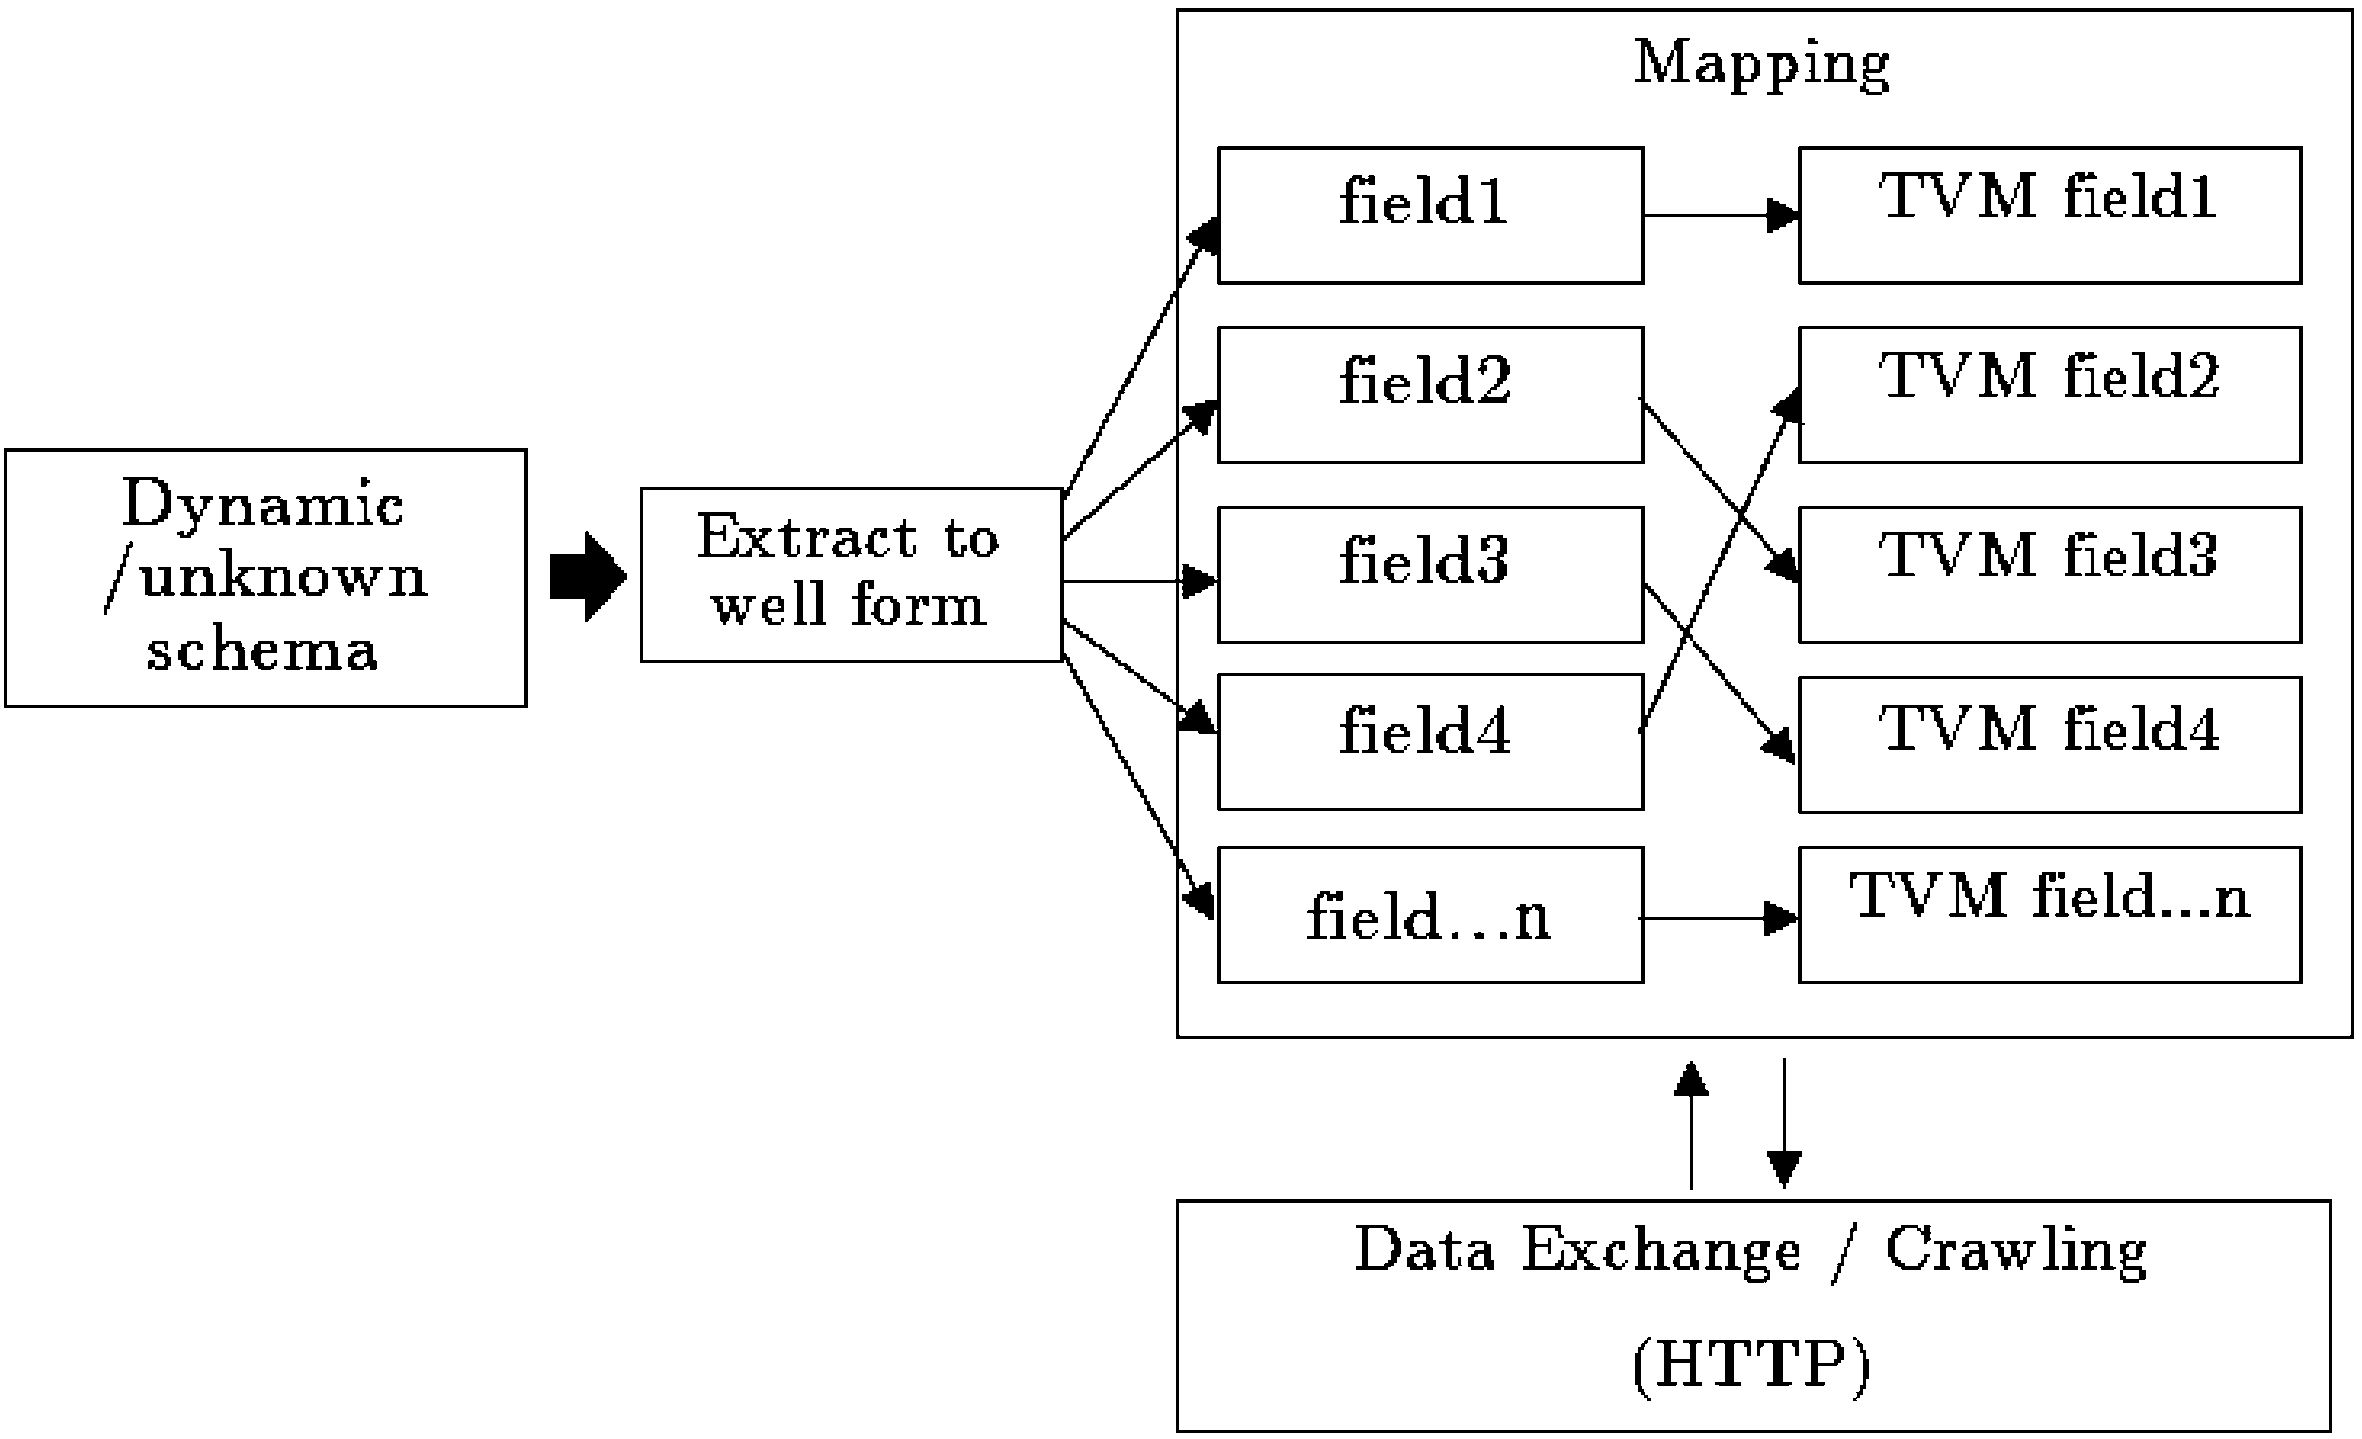
\includegraphics[scale=1]{tvmMapping}
	}
	\caption{Extracting and mapping dynamic schema to TVM schema.}\label{fig:tvmMapping}
\end{figure}

The parser service in Figure~\cref{fig:tvmMapping}, show step by step to exchange data where this service can be receiving and parsing XML or JSON format in dynamic schema includes Conceptual Interchange Documentation -- Conceptual Reference Model, Lightweight Information Describing Objects (LIDO), and Open Archives Initiative Protocol for Metadata Harvesting (OAI-PMH), however, we must define dynamic or unknown schema and extracting this schema to well form. Data exchange can be starting when the well form schema is similar with TVM schema, if not then mapping the well form schema to TVM schema should be done, only then data exchange can be performed through Hypertext Transfer Protocol (HTTP) web services.

\paragraph{4. Data store.} An important part of data-access service is storing and maintaining data collections which have been crawled and parsed to the standard data structure form. There are many techniques to preserve document collections, one of them is storing into databases. To store data from crawler service, we are using non-traditional database key- value MongoDB for handling structure, semi-structure and unstructured data. There are many advantages of MongoDB as mention in \cite{StanescuBrezovanBurdescu,JiaZhaoWang,WuChenJiang}, this type NoSQL document-oriented database using JSON-like format called Binary JSON (BSON), support for partition and MapReduce. MongoDB is using document store model, allow developer to create free-schema, running on multiplatform and opensource.

In our case we have developed a system to access MongoDB database server using Mgo (mango) driver for Go programming language. The Mgo driver is providing simple application programming interface, easy to use, and fast enough for performing task such as create, read, update, delete operations (\textit{https://labix.org/mgo}). The design of TVM database schema for museum collections \cite{AnggaiBlekanovSergeev2015} as shown in table~\cref{tab:tvmDbSchema} is independent and can be customized depend on the goals of spesific index task.

\begin{table} [htbp]%
	\centering
	\caption{TVM database schema for document collections.}%
	\label{tab:tvmDbSchema}% label всегда желательно идти после caption
	\renewcommand{\arraystretch}{1.6}%% Увеличение расстояния между рядами, для улучшения восприятия.
		\begin{adjustbox}{width=0.9\textwidth}
		\small
			\begin{tabulary}{\textwidth}{@{}>{\zz}L >{\zz}C >{\zz}C@{}}% Вертикальные полосы не используются принципиально, как и лишние горизонтальные (допускается по ГОСТ 2.105 пункт 4.4.5) % @{} позволяет прижиматься к краям
			\toprule     %%% верхняя линейка
			N & Key & NameDescription \\
			\midrule %%% тонкий разделитель. Отделяет названия столбцов. Обязателен по ГОСТ 2.105 пункт 4.4.5
			1 &  \_id &  Unique object identification \\ 
			2 & iddata & Identification of each data sources \\
			3 &  idinstitution &  Identification of museum institution\\ 
			4 & name & Object name or title \\ 
			5 & regcode & Registration code\\
			6 & category & Information about category or type of the object \\
			7 & collector & Person who collects the object \\ 
			8 & datefound & Date when the object was founded \\
			9 & placesfound & Places where the object was founded \\
			10 & period & Period or year of the object event happened \\
			11 & age & Age of the object \\
			12 & dimensions & Dimensions of the object\\
			13 & weight & Weight of the object \\
			14 & material & Materials forming or made of the object \\ 
			15 & condition & Description of past and recent object condition \\
			16 & totalcollection & Total object in the museum institution \\
			17 & description & Detail object description \\
			18 & ref & Reference information about where the data have been taken\\
			19 & creator & Creator of the document record in database\\
			\bottomrule %%% нижняя линейка
		\end{tabulary}%
	\end{adjustbox}
\end{table}

\paragraph{5. Forward index.} There are several IR techniques for document indexing system (\textit{https://www.elastic.co/blog/found-indexing-for-beginners-part3}), one of them is forward index \cite{BrinPage}, which is fast to perform task in document indexing. We are taking the museum collections data from MongoDB and managing those collections in TVM forward index. We have modified standard forward index data structure according to TVM data structure needed as shown in Figure~\cref{fig:tvmForwardIndex}.

\begin{figure}[ht]
	\centerfloat{
		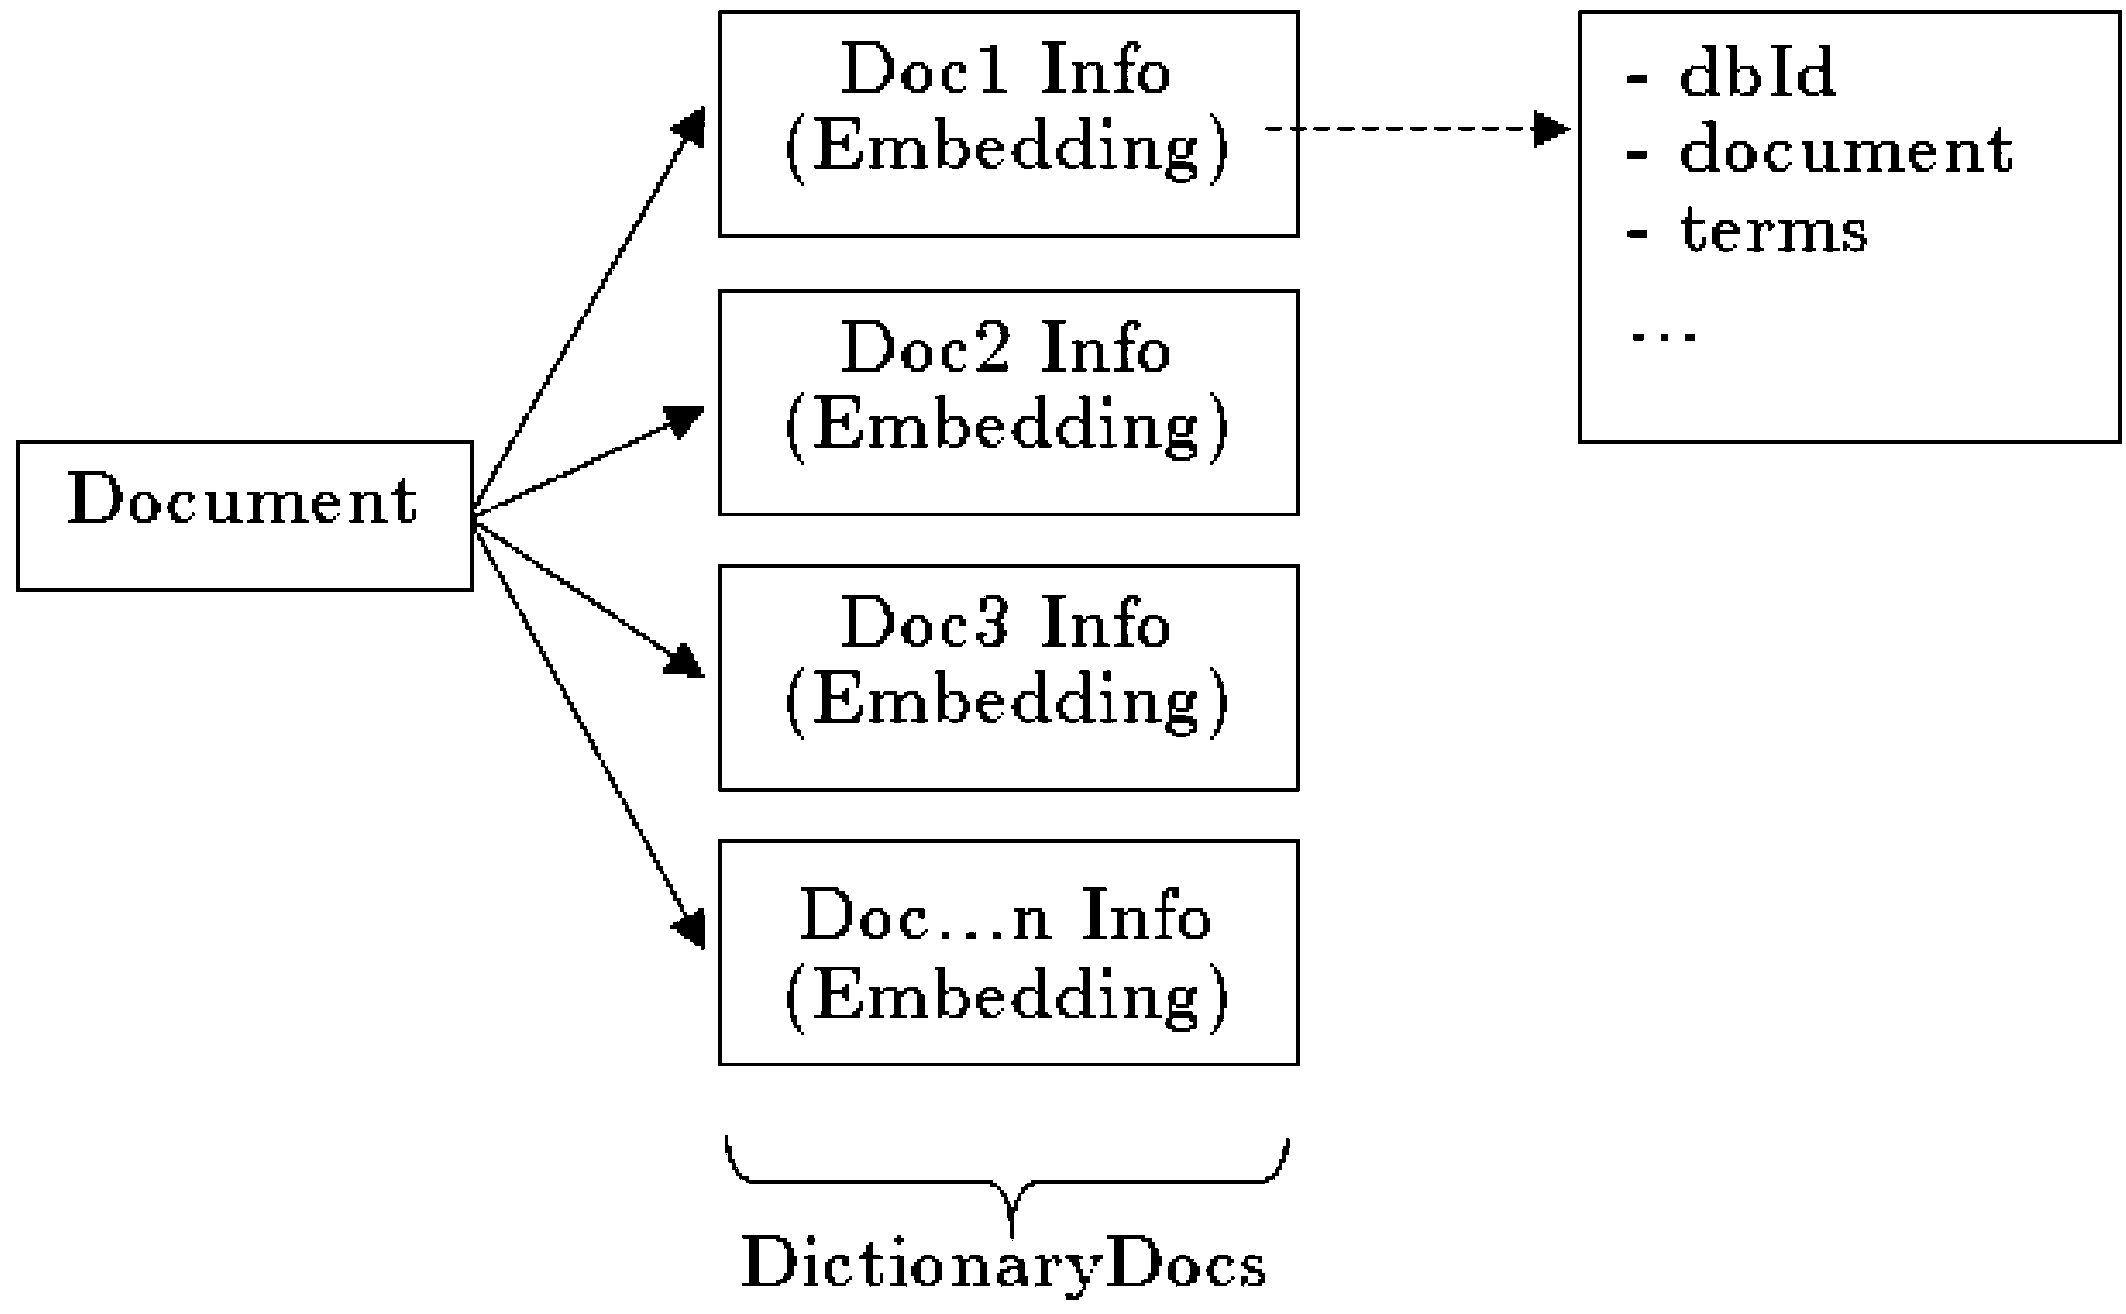
\includegraphics[scale=1]{tvmForwardIndex}
	}
	\caption{Extracting and mapping dynamic schema to TVM schema.}\label{fig:tvmForwardIndex}
\end{figure}

TVM forward index is pair document-payload using unique document identifier (DocId) for each document collections, in order to gain fast access to a document we are using hash map. Payload or embedding information in this forward index can be contains document identifier, list of terms contains in document, a record document information from database, and some necessary information. The development on flexible payload as our approach in TVM forward index give us space to embed something useful in managing and interacting with TVM inverted index.

\paragraph{6. Inverted index.} TVM concept which focus on fastest retrieving information need must be designed with good data structure, therefore we have created inverted index as a base for maintaining and searching information from any type application or users queries. There are many standard inverted index models have studied in \cite{ZobelMoffat,ManningRaghavanSchutze,PanevBerberich}, based on those state of the art we are modifying and designing inverted index structure for TVM need \cite{AnggaiBlekanovSergeev2017} as shown in Figure~\cref{fig:tvmInvertedIndex}.

\begin{figure}[ht]
	\centerfloat{
		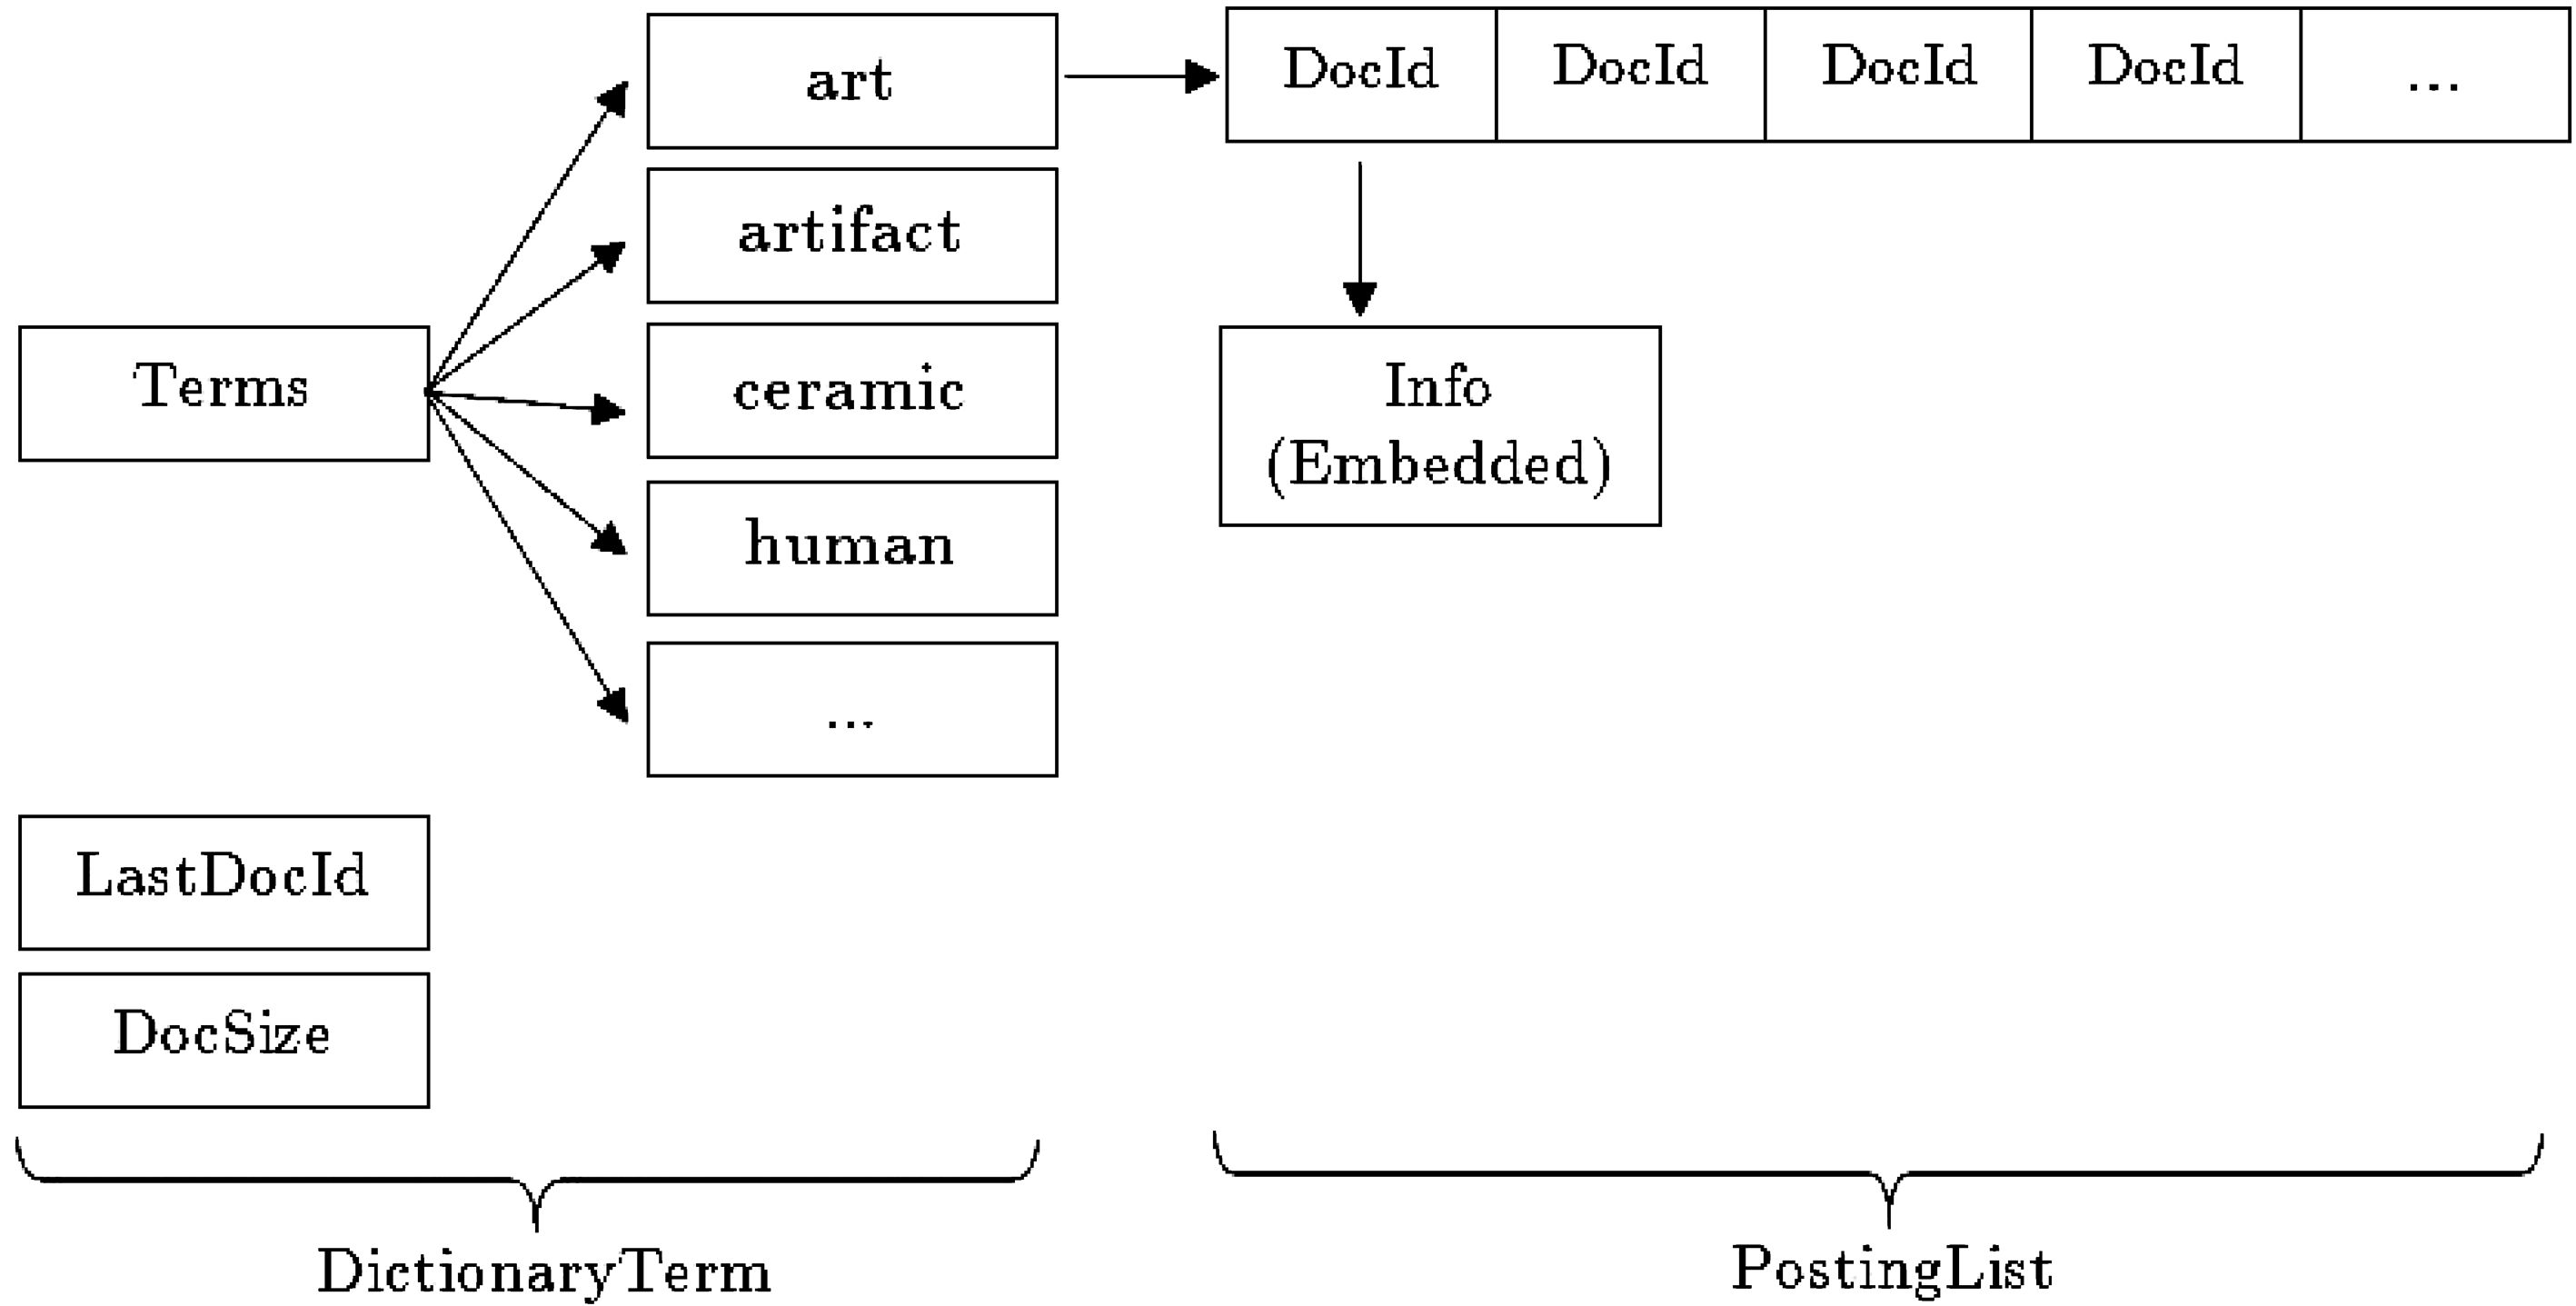
\includegraphics[scale=1]{tvmInvertedIndex}
	}
	\caption{Extracting and mapping dynamic schema to TVM schema.}\label{fig:tvmInvertedIndex}
\end{figure}

TVM inverted index maintain terms in dictionary using hash map in order to gain fast lookups, adds and deletes operations. Hash map as theoretically is performing \(O(1)\) and the worst case is \(O(n)\). Posting list for each term in dictionary also using hash map, it means that our dictionary term design is using double hash map. Access to an embedded information in this TVM inverted index will perform \(O(1)\) and the worst case is \(O(1*n)\) or \(O(n + m)\) respectively.

TVM inverted index module is providing several ranking functions such as bag of words term-frequency -- inverse document frequency (TF-IDF) \cite{ManningRaghavanSchutze}, cosine similarity measure vector space model (VSM) \cite{SaltonBuckley}, includes data provider for conceptual modeling latent semantic indexing (LSI) [9, 13] and topic modeling latent derelict allocation (LDA) \cite{BleiNgJordan}, another ranking function can be added as needed as long as it is still matching with TVM inverted index data structure design.

\paragraph{7. Microservices.} Index service in TVM are running on server side, therefore we have designed a microservices in order to communicate between applications, and serve requests from front-end to back-end server \cite{AnggaiBlekanovSergeev2015}. There are many benefits of microservice architecture as mentions in \cite{Singleton,GuoWangZeng,Bakshi}. TVM microservice in this case only support HTTP POST request with data submission to prevent security issue as shown in algorithm below:

\begin{figure}[ht]
	\centerfloat{
		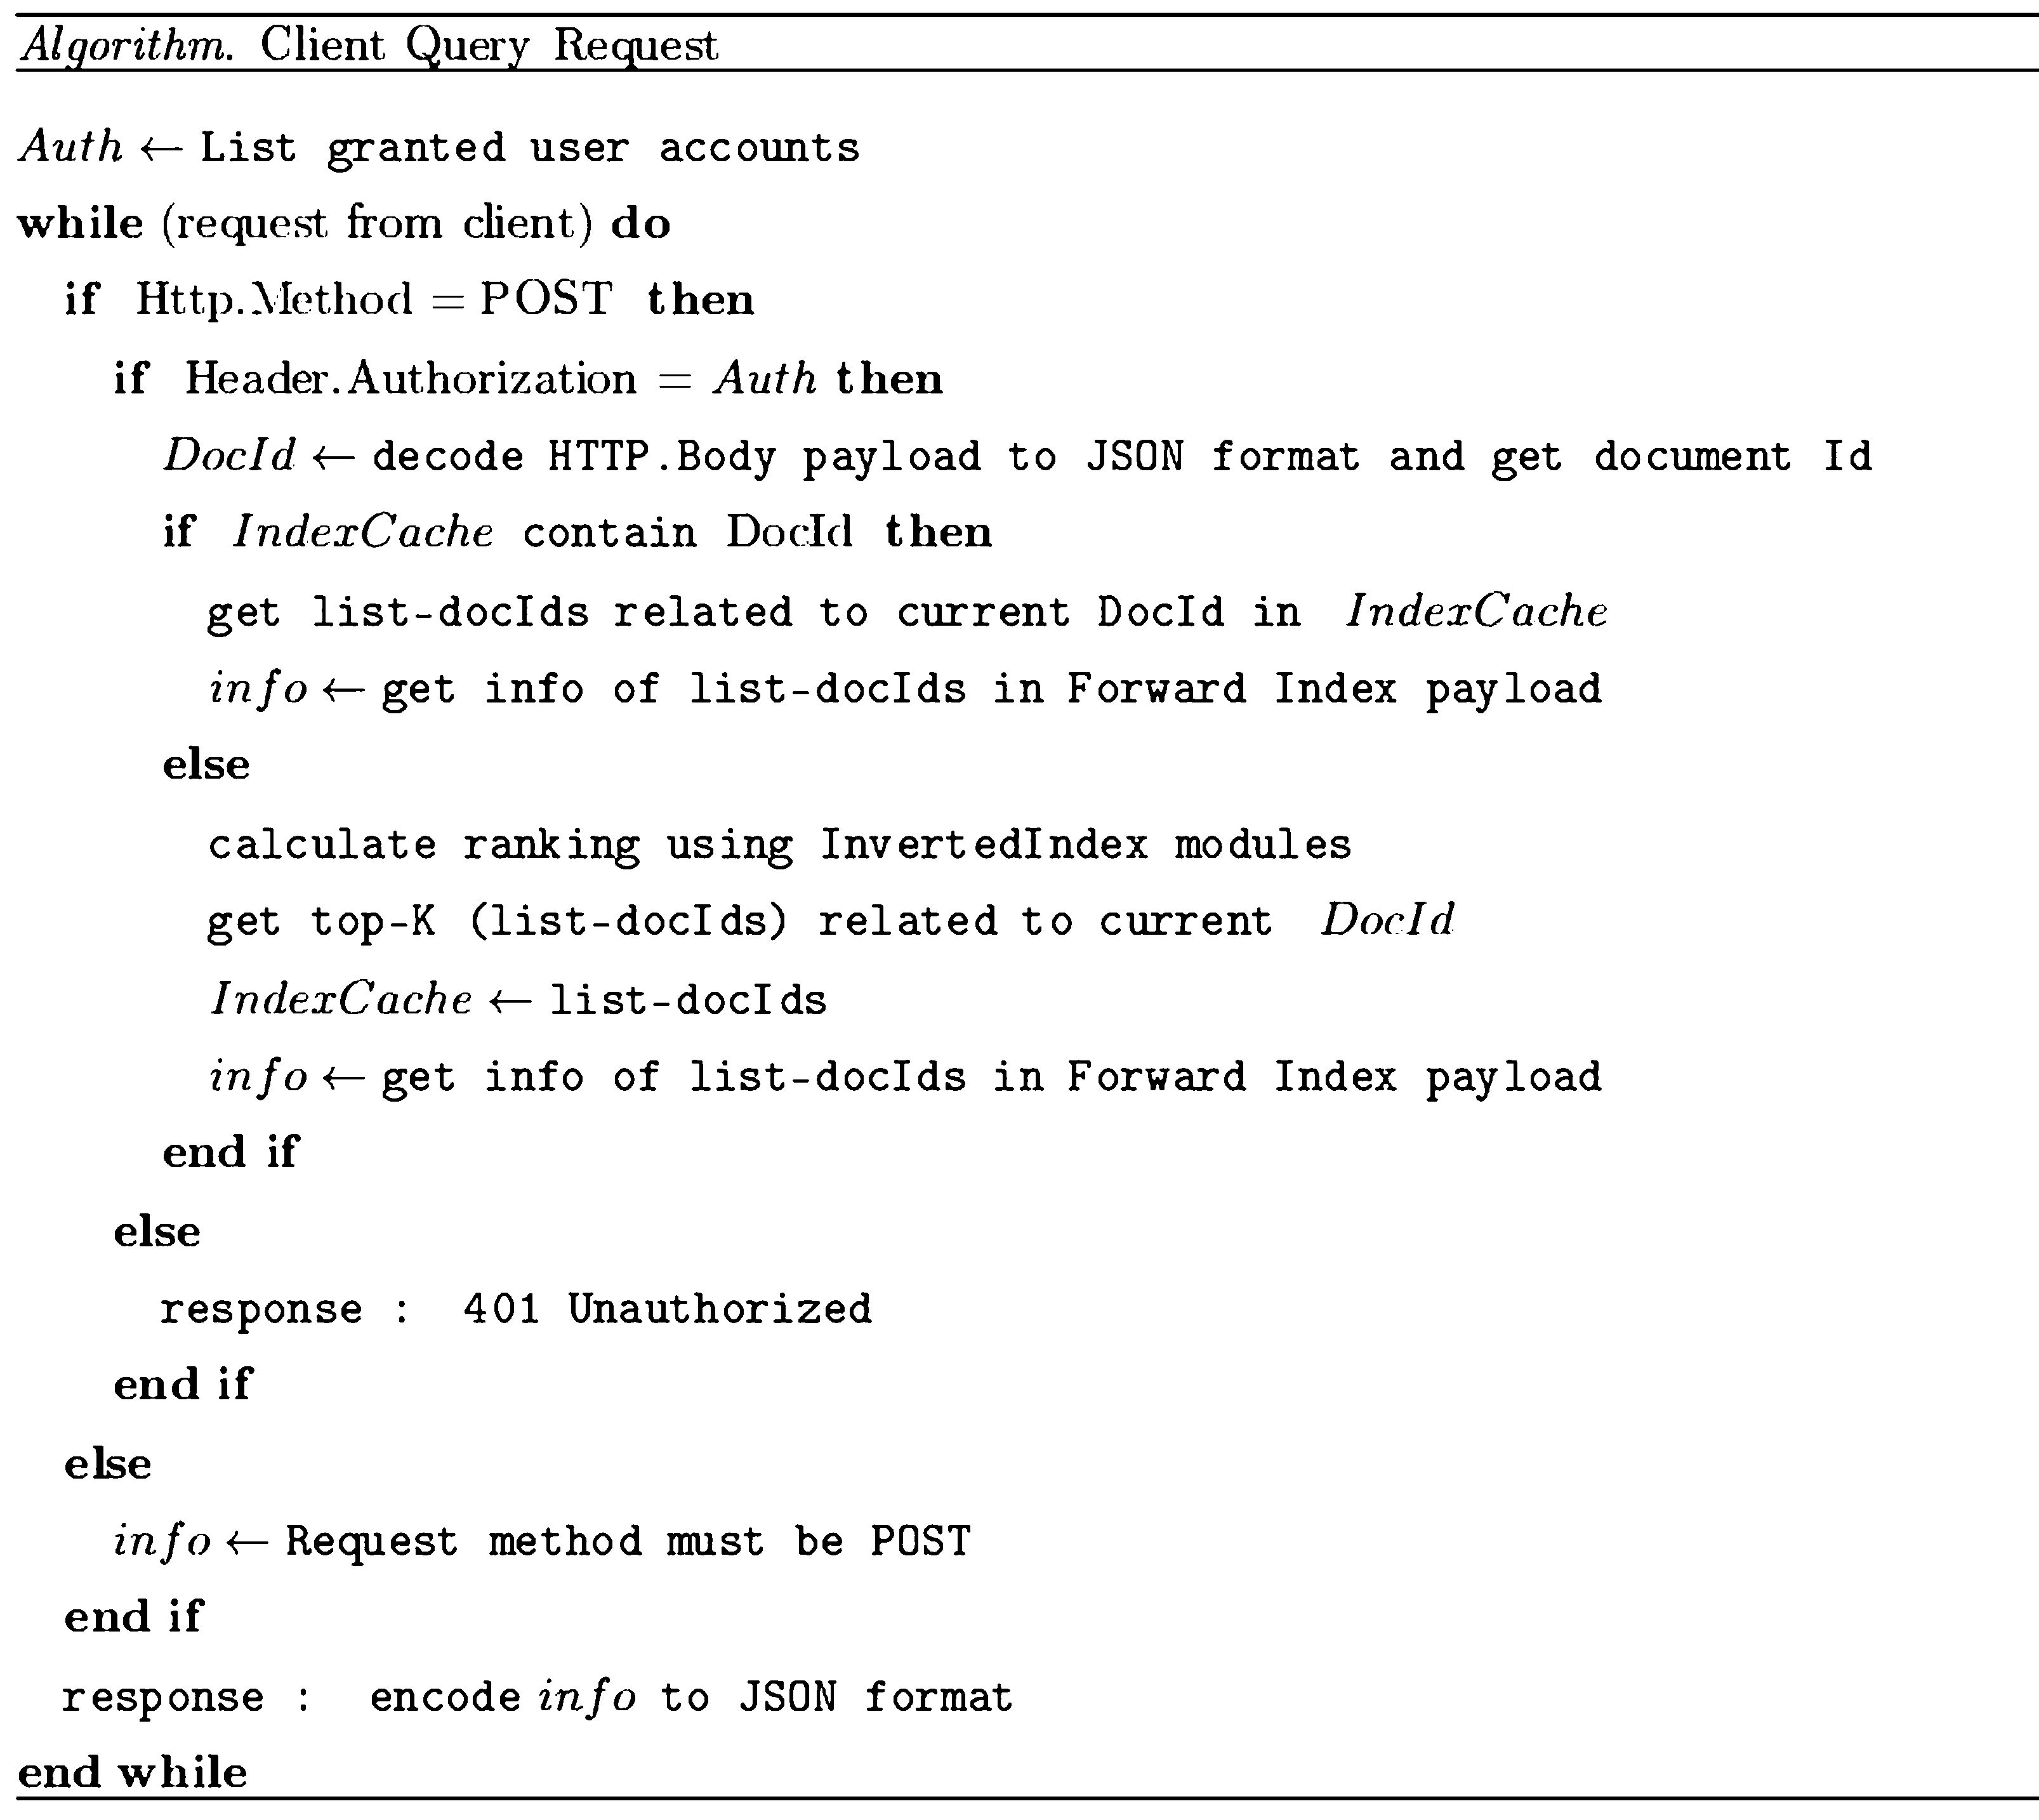
\includegraphics[scale=1]{algoQuery}
	}
	\label{fig:algoQuery}
\end{figure}

Algorithm pseudocode is describing how TVM microservice listening requests from clients, processing the request and give back a response in appropriate JSON format. HTTP header authentication schema is Basic, which transmit user and password credentials when the connection has established. The client request for searching similarity document is identified by DocId where each request will trigger inverted index ranking function and return list-docIds no more than maximum top-K ranked. The list-docId will be adding to the index-cache and using it again on the similar DocId request for reducing similar calculation process.

\paragraph{8. Experiment and results.} TVM system which have provided a design for microservices in this experiment will be used for handling many requests from front-end to back-end server. We have used Intel Xeon Processor 2620v4, memory DDR4 32 Gb, and hard disk Skyhawk Surveillance 2 terabyte in conducting this experiment. The data we have been using as dataset are from “Collection Museum Registration System”, Directorate Cultural Heritage Preservation and Museum, Ministry of Education and Culture, The Republic of Indonesia, which contain 29 362 collections.

In this experiment we have prepared three methods which all outputs will be encoded, written and return to the client side in JSON format, first the service will return only list of docIds form to the client in consequently allowing them to process those list of docIds for another tasks, second the service will get the list of docIds and using them as keys to identify full detail collections information in TVM forward index payload, third the service will get the list of docIds and using them to perform a query to database mongoDB for searching the detail collections information. The query request method to indicate service performance is using document at a time (DAAT) as shown in Figure~\cref{fig:daatQuery}.

\begin{figure}[ht]
	\centerfloat{
		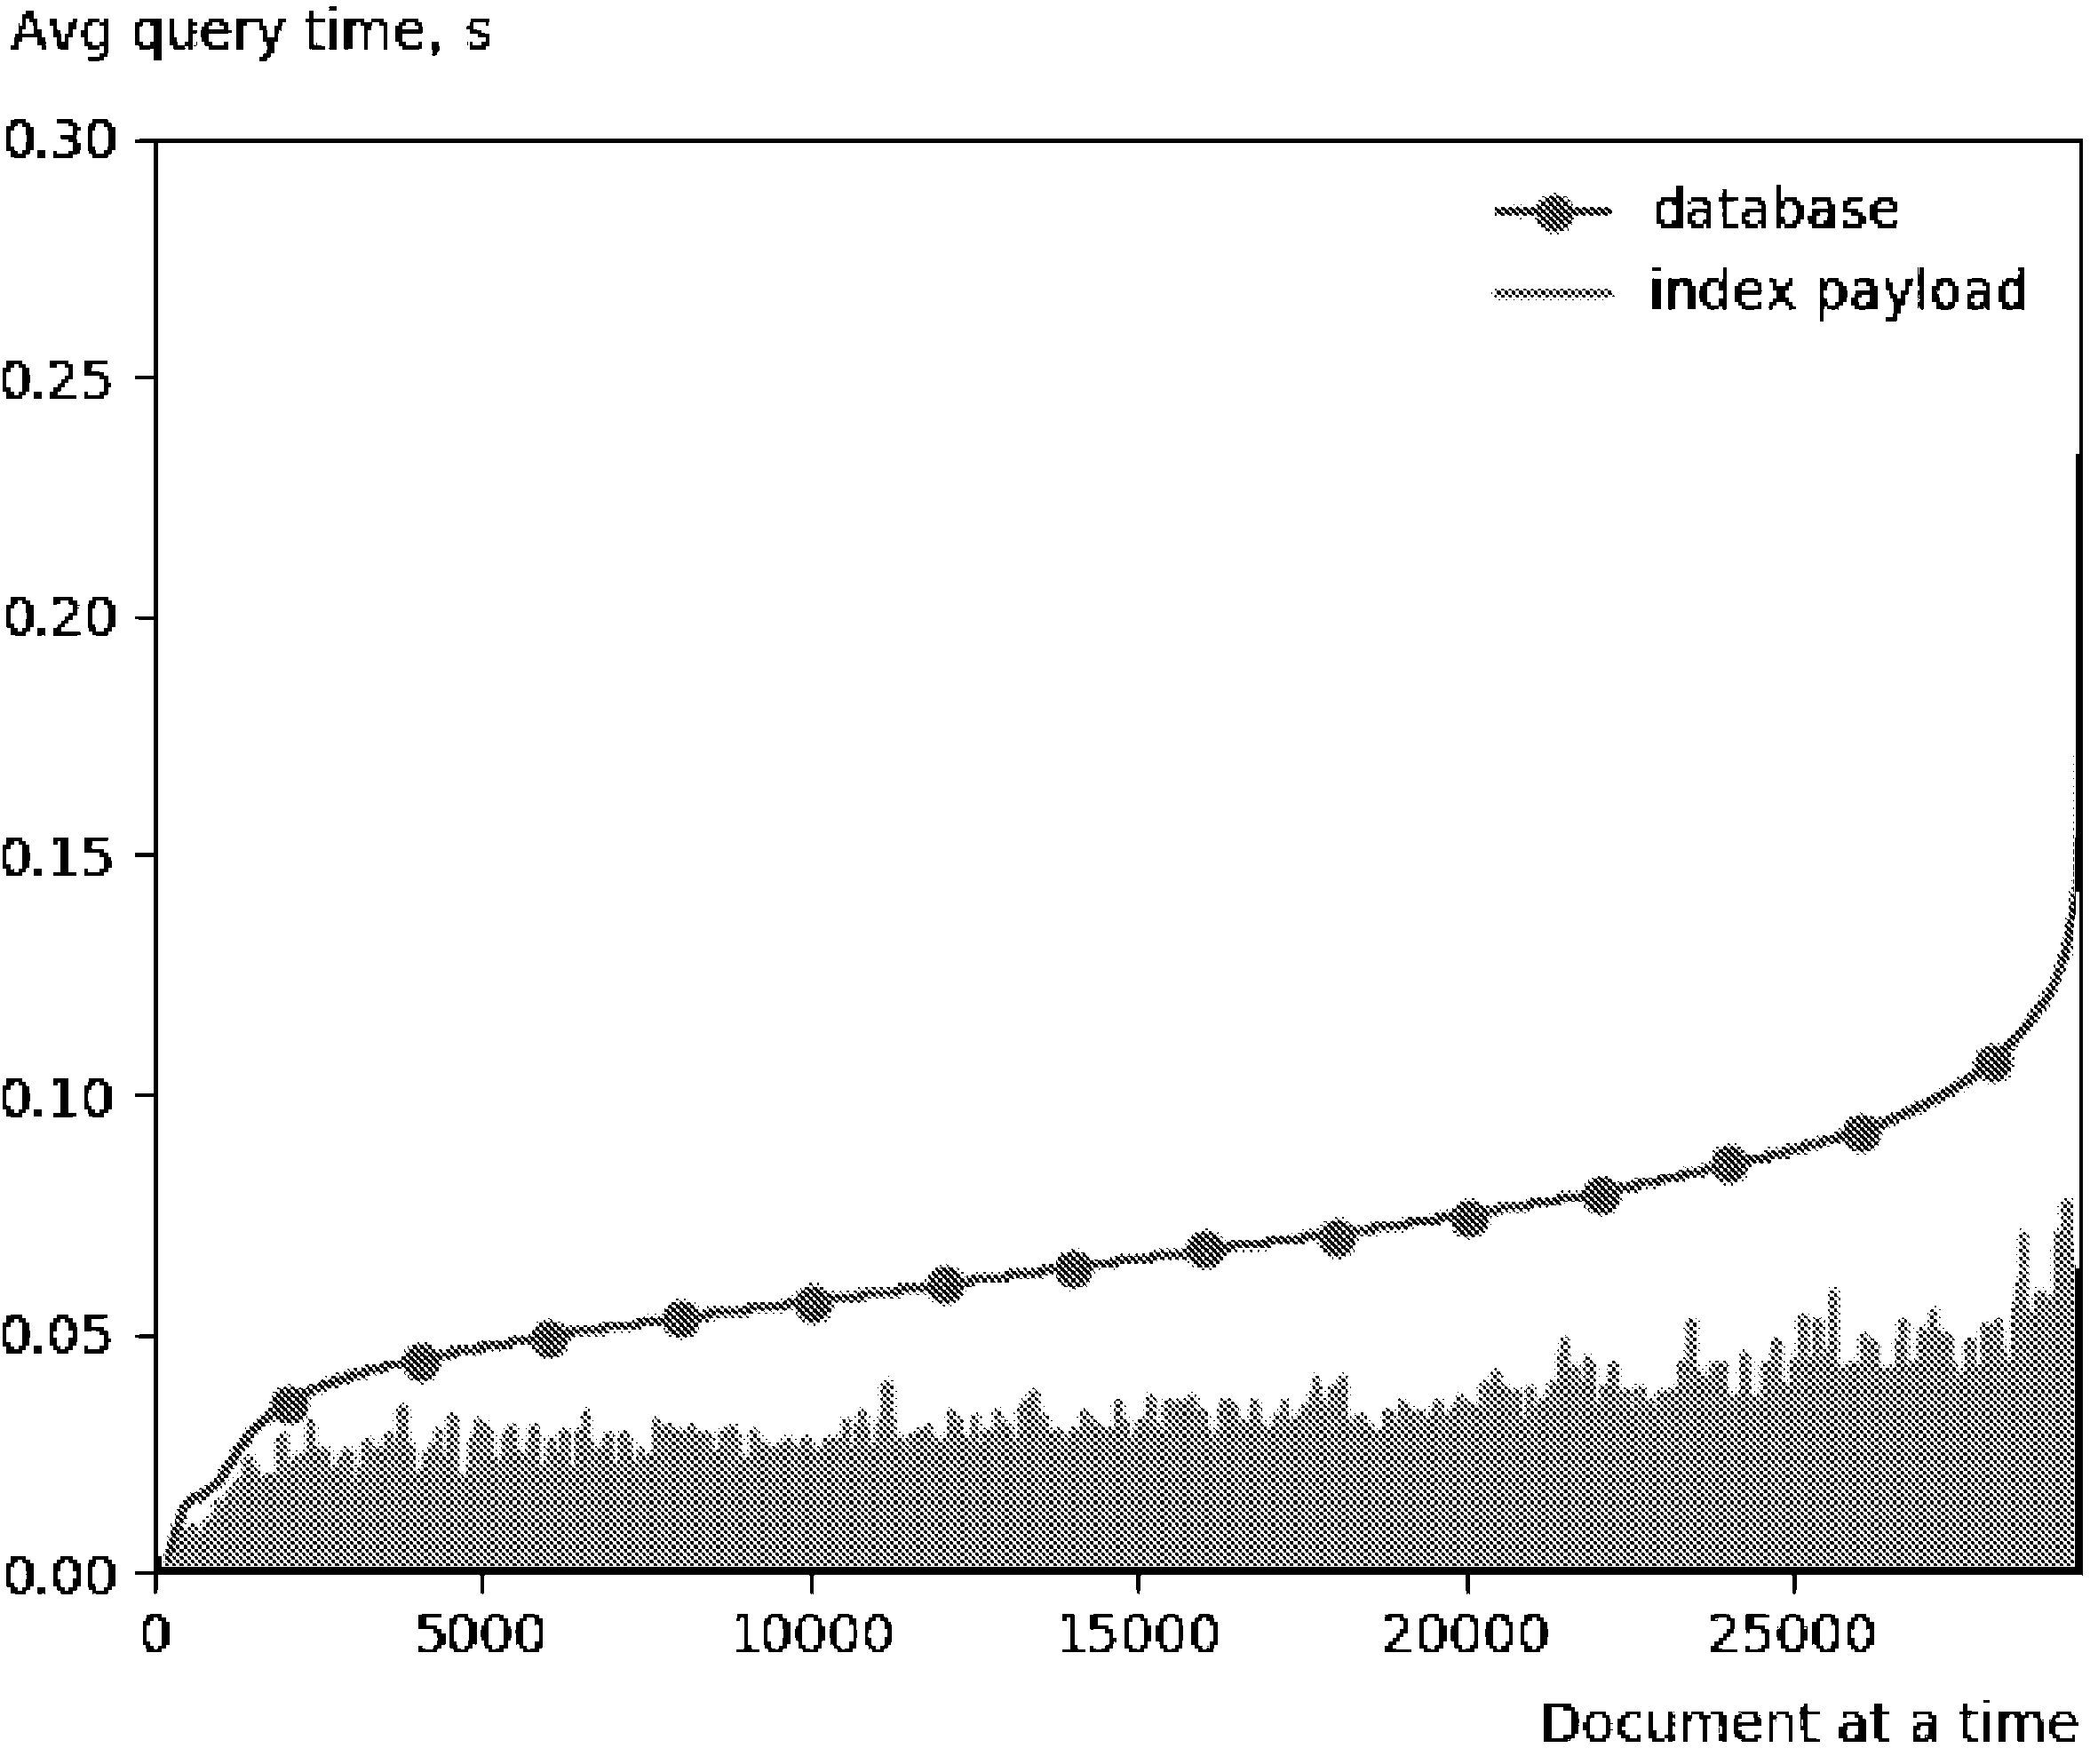
\includegraphics[scale=1]{daatQuery}
	}
	\caption{DAAT query requests from front-end to back-end server.}\label{fig:daatQuery}
\end{figure}


DAAT query request from client or front-end using appropriate JSON structure in Figure 4 was handled by TVM independent microservices where after query has performed, then inverted index function directly calculates documents score and the function returned list of top-K ranking in list of docIds form. The query processing time for accessing information to database is 84.5\% and access to index payload only need 0.02\% from total query request time.

The second experiment, we are using query term at a time (TAAT), where each term in TVM inverted index dictionary have been using for query requests in order to evaluate and calculating documents score which have contained in postings list. The result as shown in Figure~\cref{fig:taatQuery} is describing query time to database need 99.4\% and query to TVM index payload only 0.0005\% from total query request time.

\begin{figure}[ht]
	\centerfloat{
		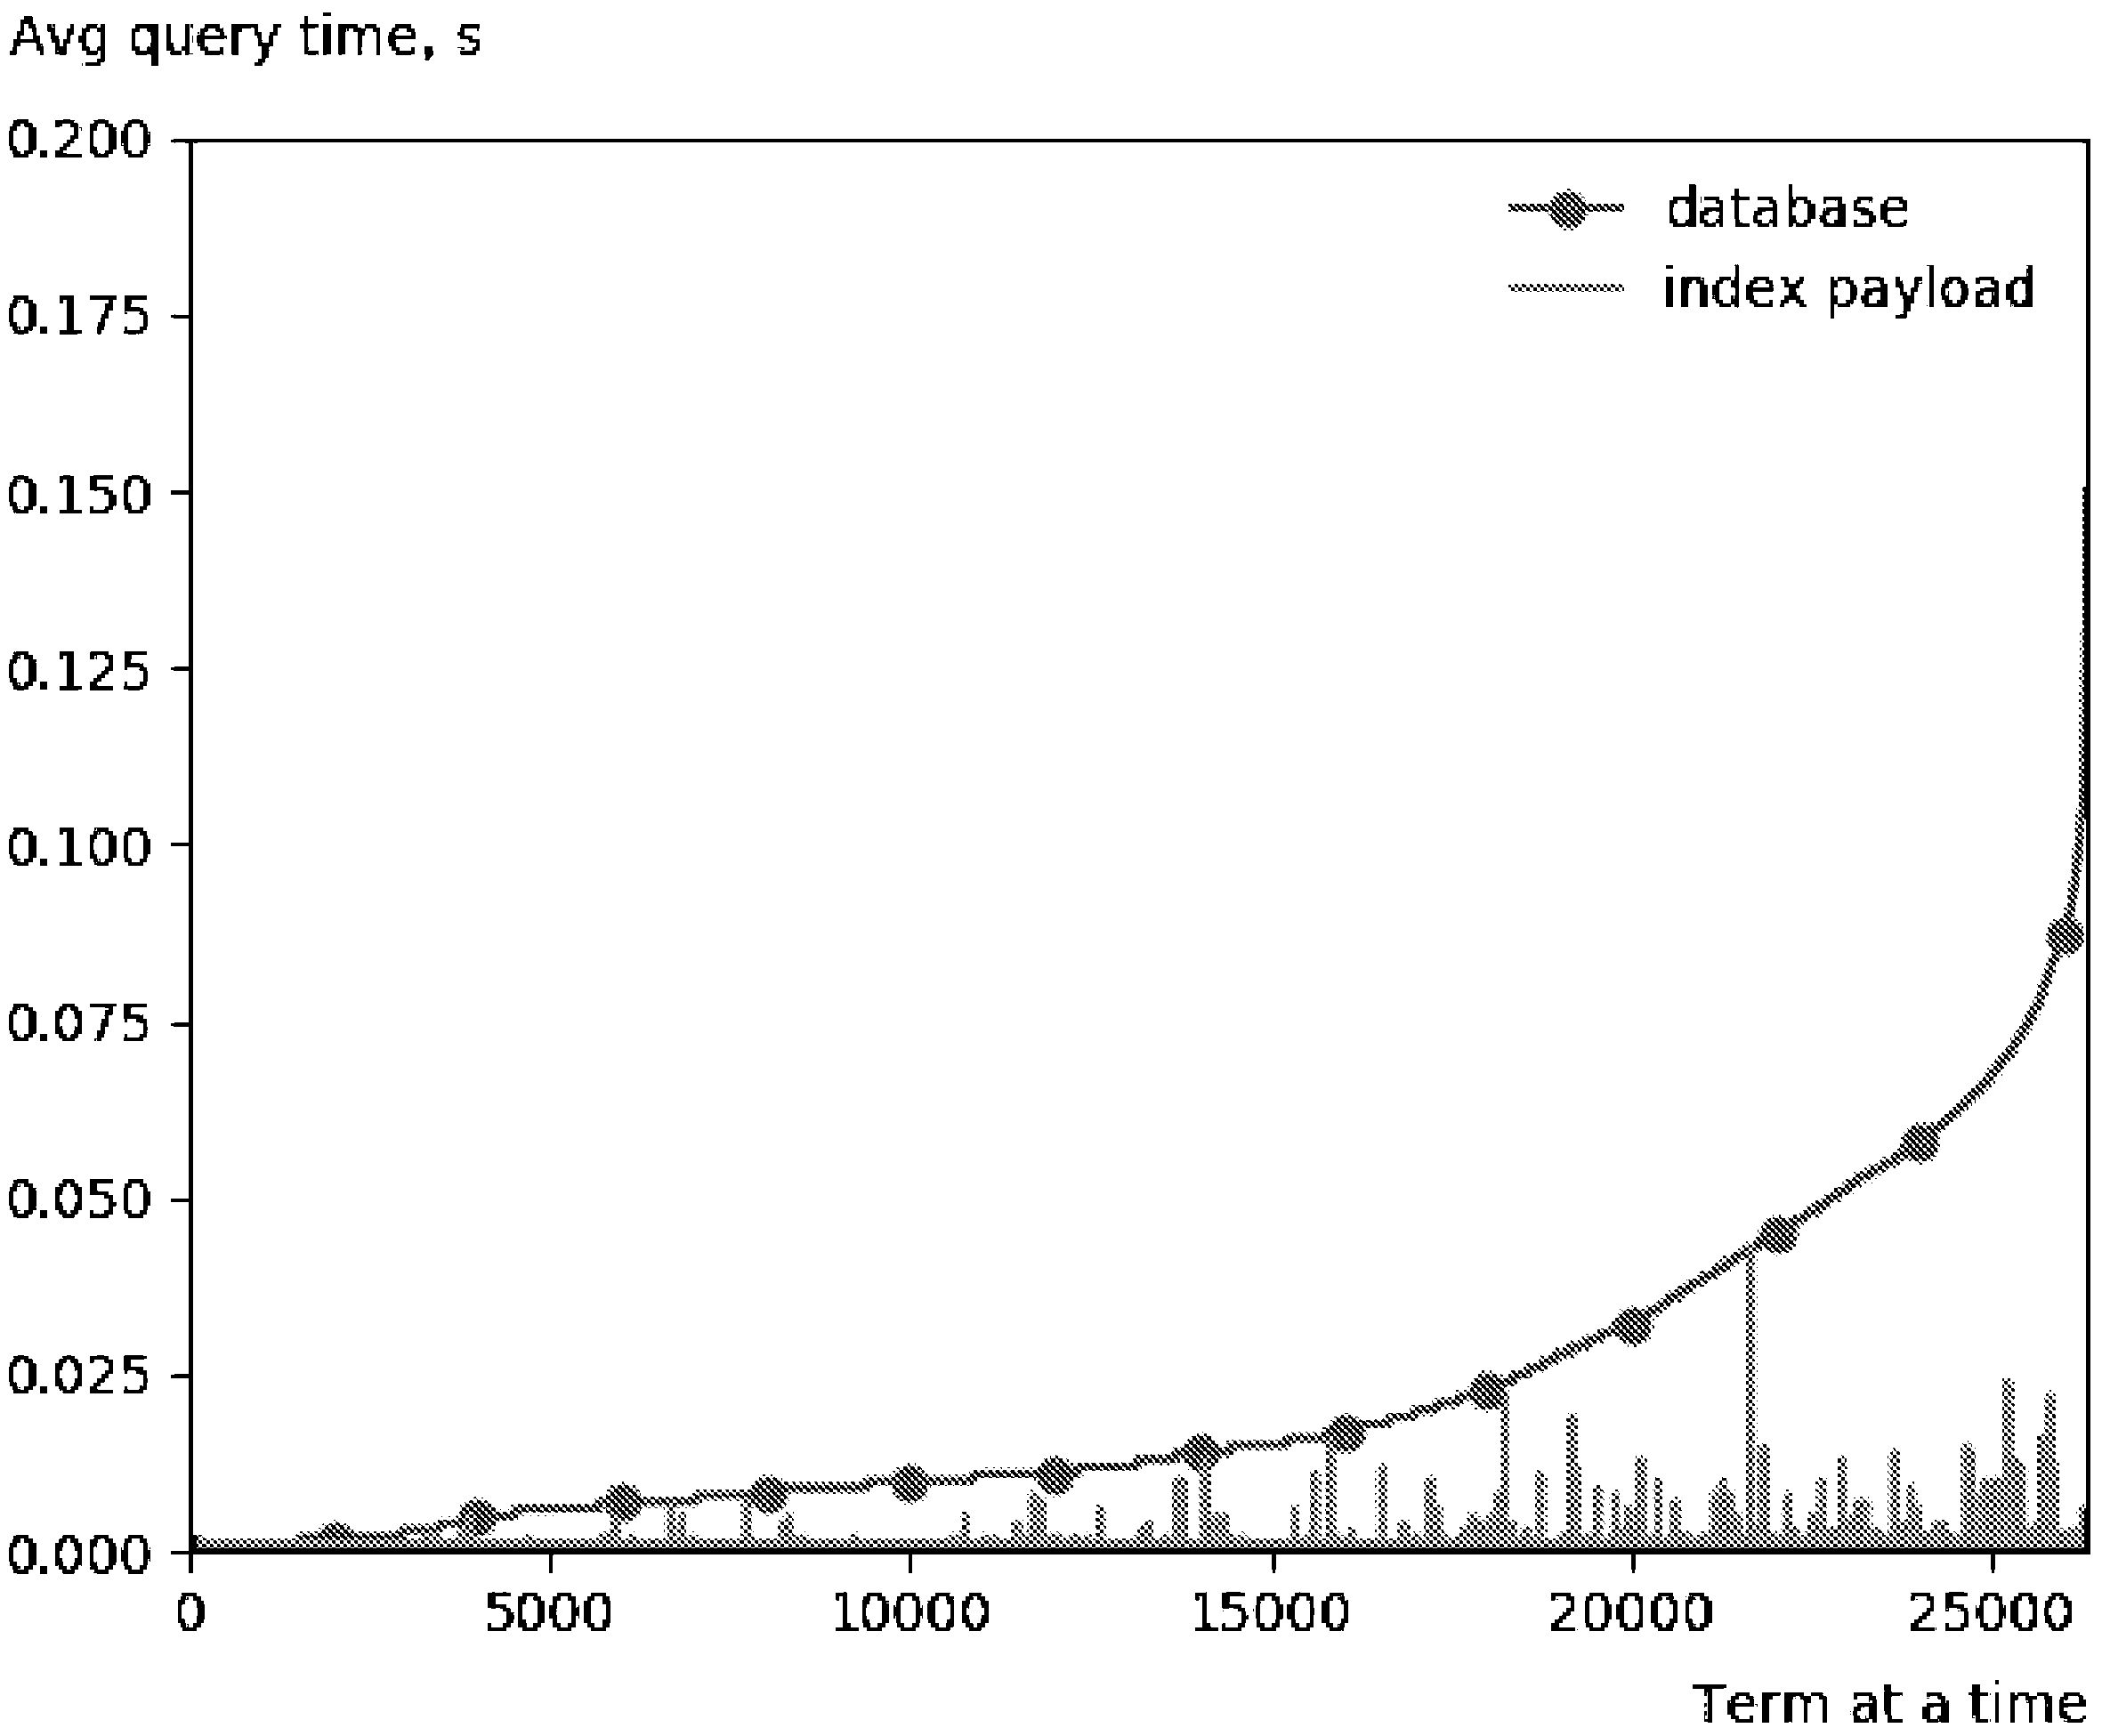
\includegraphics[scale=1]{taatQuery}
	}
	\caption{TAAT query requests from front-end to back-end server}\label{fig:taatQuery}
\end{figure}

The first method is only gives docIds list rather than give a full information, therefore there is no request needed to database or index payload, beside this docIds list can be used as caching for top-K docIds ranking in order to reduce computation time in back-end server. The cache key is docId of recent document which is using as query request, and the value is containing array set of documents identification. The second and third methods give us a significant result, where our method have provided an access to collaborate between TVM inverted index and forward index by given embedded information as payload. Our experiments shown that the methods have been proposed can reduced time to access a detail information of the collection rather than given many direct queries to database system.

\paragraph{9. Conclusion}. In this work we have constructed data access service, modified forward and inverted index, and design special microservice architecture for TVM to provide relevant information for the virtual museums visitors. There are several experiments we have conducted, and shown our methodology give significant results when exchanged an information and collaborated between TVM forward and inverted index, query request, process and response through microservices give high performance output. Dynamic or flexible payload in TVM indices structure can be used for multipurpose indexing method in the development of modern information retrieval.


\section{Оптимальное конструирование сборщика (цепочка роботов)}\label{sec:ch4/sect3}

\section{Реализация программного комплекса}\label{sec:ch4/sect4}

\FloatBarrier

